\chapter{Architectural Details of ``Sapphire Rapids'' Processors}
The Sapphire Rapids family of server processors is the successor to the ``Ice Lake'' architecture.
It is the first in Intels lineup of server processor to introduce a modular design containing four tiles in a 2x2 grid interconnected with EMIB structures.
The two variants of this processor are the 4th Generation Intel Xeon Scalable Processor and Xeon CPU Max Series with four additional HBM blocks~\cite{Intel_2021_Hotchips}.
Each tile contains up to 15 Golden Cove cores with a shared L3 cache connected by a mesh, an accelerator complex, two DDR5 memory busses, TODO PCIe Gen 5 and one UPI 2.0 link.
This structure enables the package to be used in a single memory domain or split into two or four sub-NUMA clusters~\cite{Intel_4th_gen_scalable}.
Each accelerator complex can contain contain up to four different accelerators.
Data Streaming Accelerator (DSA) allows for memory move, fill and compare offloading.
QuickAssist Technology (QAT), allows for acceleration of cryptographic operations.
Dynamic Load Balancer (DLB), brings hardware acceleratored queues.
In-Memory Analytics Accelerator (IAA), allows for memory compression, encryption and filtering.~\cite{Yifan_2024_intel_accelerator_ecosystem,Yuan_2023_ISCA_tutorial,Intel_4th_gen_scalable}
Which accelerators are activated depend on the specific SKU, while Intel allows for the option to install licenses through an PCI express interface\footnote{\url{https://github.com/intel/intel-sdsi}}~\cite{Krenn_2025_Intel_on_demand}.

\todoms{Information about the PCIe and DDR5}

\begin{figure}[]
    \centering
    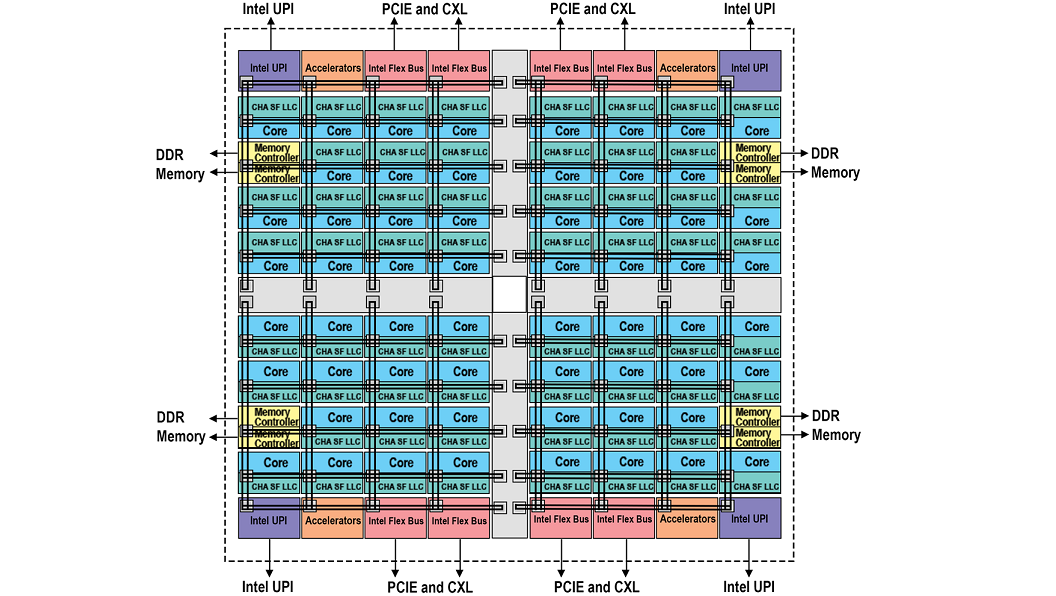
\includegraphics[width=\columnwidth]{fig/spr-uma.png}
    \caption{Block diagram of the 4th Generation Intel Xeon Scalable Processor from~\cite{Intel_4th_gen_scalable}.
Two mirrored tiles are arranged in a 2x2 grid, which are interconnected with EMIB structures to continue the mesh across the die boundaries.~\cite{Intel_2022_ISSCC}}
\end{figure}

\todoms{Show test system detail table.}

\section{Golden Cove Core Microarchitecture}

\begin{figure}[]
    \centering
    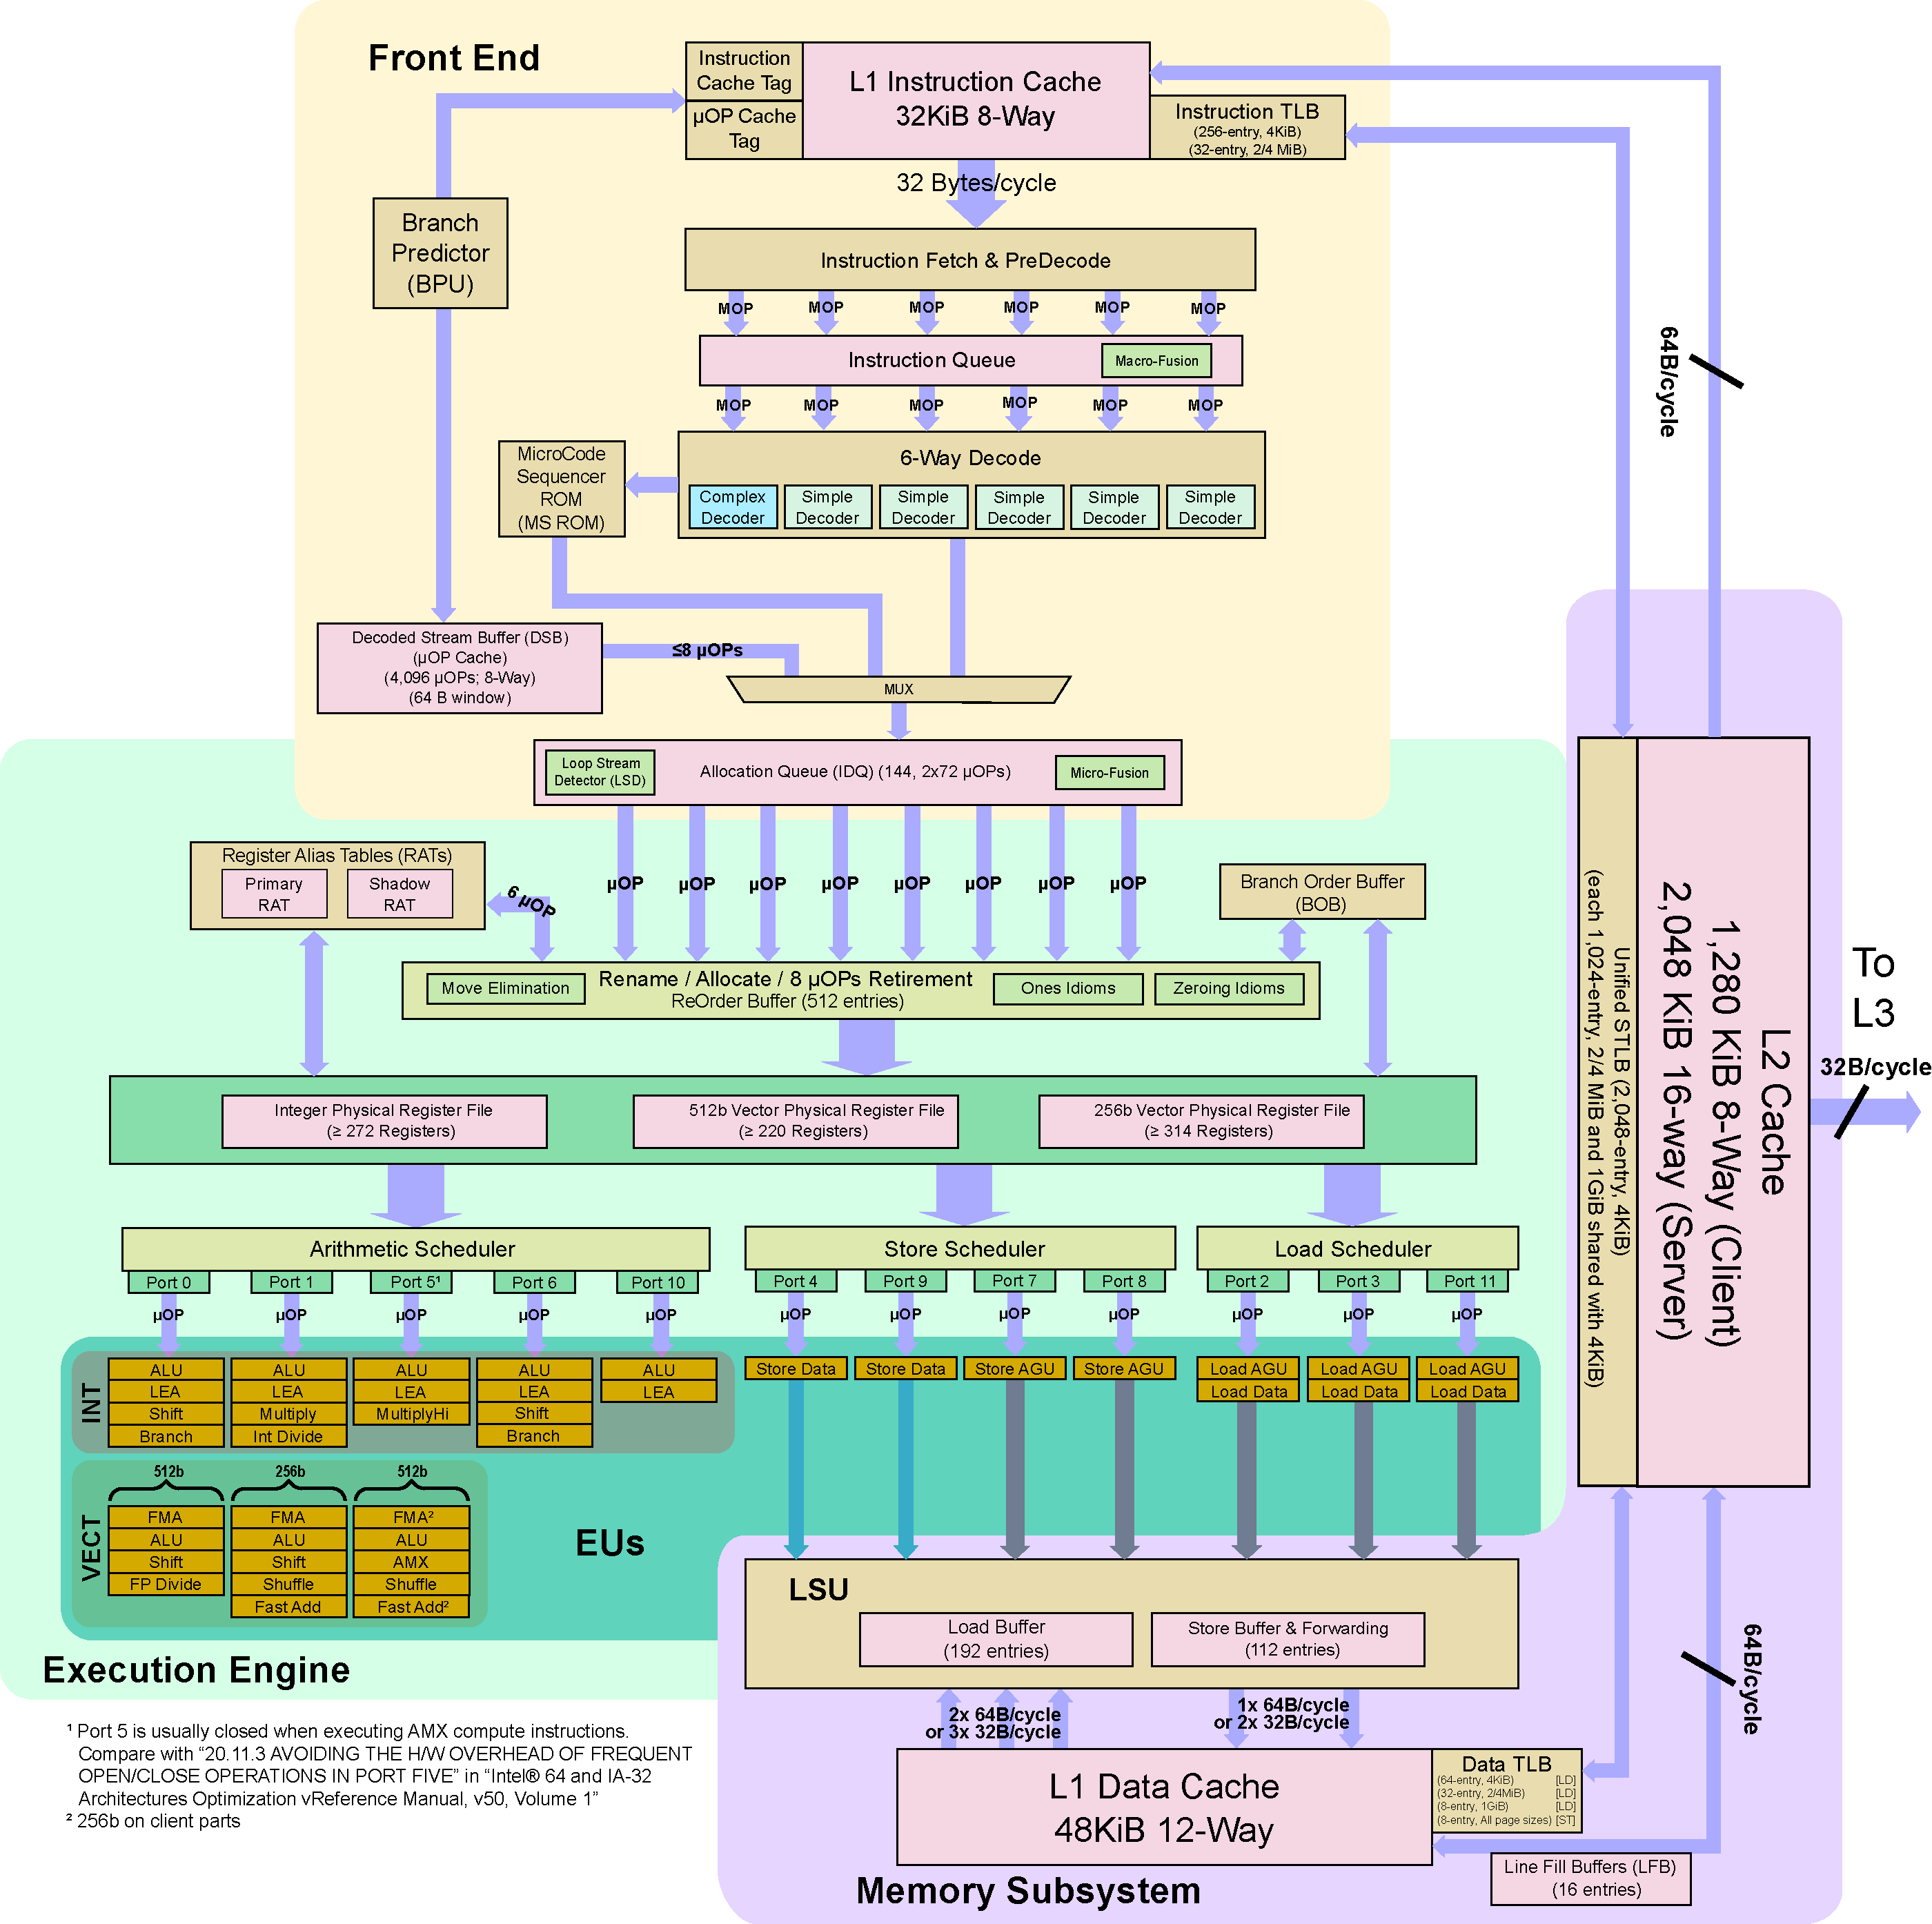
\includegraphics[width=\columnwidth]{fig/GoldenCoveCore.pdf}
    \caption{Block diagram of the Golden Cove Core.}
    \todoms{Measurements for the schedulers. How did the frontend change? Details of port 5 closing.}
\end{figure}